\documentclass[aspectratio=169]{beamer}
\usepackage{colortbl,tabularx,mathrsfs,calligra}
\usepackage{amsmath,amsfonts,amssymb,amsthm}
\usepackage{ragged2e}
\usepackage{tikz}
\usepackage{caption}
\usepackage{wrapfig}
\usepackage{multirow}
\usepackage{multicol}
\usepackage{array}
\usepackage{pgfplots, tkz-euclide,calc}
    \pgfplotsset{compat=1.18}
\usepackage{listings}

\graphicspath{{C:/Users/teoso/OneDrive/Documents/Tugas Kuliah/Template Math Depart/}{./foto/}}

\definecolor{HIMAmuda}{HTML}{01D1FD}
\definecolor{HIMAtua}{HTML}{02016A}
\definecolor{HIMAabu}{HTML}{CBCBCC}

\usetheme{Madrid}

\setbeamercolor{palette primary}{bg=HIMAtua,fg=white}
\setbeamercolor{palette secondary}{bg=HIMAmuda,fg=black}
\setbeamercolor{palette tertiary}{bg=HIMAabu,fg=black}
\setbeamercolor{palette quaternary}{bg=HIMAmuda,fg=white}
\setbeamercolor{structure}{fg=HIMAmuda} % itemize, enumerate, etc
\setbeamercolor{section in toc}{fg=HIMAtua} % TOC sections
\setbeamercolor{bibliography item}{parent=palette secondary}
\setbeamercolor*{bibliography entry author}{parent=section in toc}
\setbeamercolor{framesubtitle}{fg=HIMAmuda} % Hanya warna teks subtitle


\usetikzlibrary{shapes.geometric, arrows}

\tikzstyle{startstop} = [ellipse, minimum width=1cm, minimum height=1cm,text centered, draw=black, fill=red!30]
\tikzstyle{process} = [rectangle, minimum width=2cm, minimum height=1cm, text centered, draw=black, fill=blue!30]
\tikzstyle{decision} = [diamond, minimum width=1cm, minimum height=1cm, text centered, draw=black, fill=blue!50]
\tikzstyle{arrow} = [thick,->,>=stealth]

\newcolumntype{L}[1]{>{\raggedright\let\newline\\\arraybackslash\hspace{0pt}}m{#1}}
\newcolumntype{C}[1]{>{\centering\let\newline\\\arraybackslash\hspace{0pt}}m{#1}}
\newcolumntype{R}[1]{>{\raggedleft\let\newline\\\arraybackslash\hspace{0pt}}m{#1}}

\usefonttheme{professionalfonts}
\setbeamertemplate{theorems}[numbered]
% \setbeamercovered{transparent}


\theoremstyle{definition}
% \numberwithin{subsection}{section}
\newtheorem{definisi}{Definisi}
\newtheorem{teorema}{Teorema}
\newtheorem{soal}{Soal}
\newcommand{\R}{\mathbb{R}}
\newcommand{\N}{\mathbb{N}}
\newcommand{\Z}{\mathbb{Z}}
\newcommand{\C}{\mathbb{C}}
\newcommand{\Q}{\mathbb{Q}}

\AtBeginEnvironment{definisi}{
    \setbeamercolor{block title}{fg=white,bg=HIMAtua}
    \setbeamercolor{block body}{parent=normal text,bg=HIMAtua!30!white}
    \setbeamercolor{item}{fg=HIMAtua}
}
\AtBeginEnvironment{teorema}{
    \setbeamercolor{block title}{bg=darkgray,fg=white}
    \setbeamercolor{block body}{parent=pallette tertiary,bg=HIMAabu!30!white}
    \setbeamercolor{item}{fg=darkgray}
}
\AtBeginEnvironment{soal}{%
  \setbeamercolor{block title}{fg=white,bg=teal} 
  \setbeamercolor{block body}{parent=normal text,bg=teal!30!white} 
  \setbeamercolor{item}{fg=teal}
}

\date{Rabu, 9 April 2025}
\title[Pengantar Analisis Fungsional]{Pembahasan Kuis 1 Pengantar Analisis Fungsional T.A 2024/2025}
\author[Teo]{Teosofi Hidayah Agung\\5002221132}
\institute[Matematika ITS]{Departemen Matematika\\ Institut Teknologi Sepuluh Nopember}
\titlegraphic{\includegraphics[scale=0.15]{logoITS}$\quad$\includegraphics[scale=0.024]{M.png}}

\begin{document}

    \begin{frame}
        \titlepage
\end{frame}

\subsection{Nomor 1}
\section{Pembahasan Soal}
\begin{frame}
  \frametitle{\insertsection}
  \begin{soal}
    Jika $A$ subspace dari $\ell^\infty$ yang terdiri dari semua barisan yang elemen-elemennya nol dan satu, maka dapatkan metrik terinduksi (induced metric) pada $A$.
  \end{soal}
  \begin{definisi}
    Ruang \( \ell^\infty \) didefinisikan sebagai himpunan semua barisan bilangan real (atau kompleks) \( x = (x_n)_{n=1}^\infty \) yang \textbf{terbatas}, yaitu:

    \[
    \ell^\infty = \left\{ (x_n)_{n=1}^\infty \,\middle|\, \sup_{n \in \mathbb{N}} |x_n| < \infty \right\}.
    \]
    
  \end{definisi}
\end{frame}


\begin{frame}
  \frametitle{\insertsection}
  \framesubtitle{\insertsubsection}
  \textbf{Jawaban:}\\
  Misalkan $x_n, y_n \in A$, maka kita dapat didefinisikan fungsi jarak $d: A \times A \to \mathbb{R}$ sebagai berikut:
  \begin{align*}
    d(x_n, y_n) &= \sup_{n \in \mathbb{N}} |x_n - y_n| 
  \end{align*}
  Lebih lanjut, karena barisan $x_n$ dan $y_n$ adalah barisan yang elemen-elemennya nol dan satu, maka berakibat 
  \begin{align*}
    \sup_{n \in \mathbb{N}} |x_n - y_n| &= \begin{cases}
      0 & \text{ jika } x_n = y_n\\
      1 & \text{ jika } x_n \neq y_n
    \end{cases}
  \end{align*}
\end{frame}

\begin{frame}
  \frametitle{\insertsection}
  \framesubtitle{\insertsubsection}
  Dengan demikian, kita dapat menyimpulkan bahwa $d$ merupakan metrik pada $A$ atau lebih tepatnya disebut \textbf{metrik diskrit}. Sehingga
  \begin{align*}
    d(x_n, y_n) &= \begin{cases}
      0 & \text{ jika } x_n = y_n\\
      1 & \text{ jika } x_n \neq y_n
    \end{cases}
  \end{align*}
  merupakan metrik terinduksi pada $A$.
\end{frame}

\subsection{Nomor 2}
\begin{frame}
  \frametitle{\insertsection}
  \begin{soal}
    Dapatkan barisan yang konvergen ke nol, tetapi bukan anggota dari $\ell^p$, $1 \leq p < \infty$. Jelaskan jawaban anda.
  \end{soal}
  \begin{definisi}
    Ruang \( \ell^p \) untuk \( 1 \leq p < \infty \) didefinisikan sebagai:

    \[
    \ell^p = \left\{ x = (x_n)_{n=1}^\infty \,\middle|\, \sum_{n=1}^\infty |x_n|^p < \infty \right\}.
    \]
  \end{definisi}
\end{frame}


\begin{frame}
  \frametitle{\insertsection}
  \framesubtitle{\insertsubsection}
  \textbf{Jawaban:}\\
  Perhatikan barisan \( x_n = \left( \dfrac{1}{\ln(n+1)} \right)_{n=1}^\infty \). Jelas bahwa \( x_n \to 0 \) ketika \( n \to \infty \). Sekarang akan dibuktikan bahwa \( x_n \notin \ell^p \) untuk \( 1 \leq p < \infty \).
  \begin{teorema}
    Jika $\displaystyle\lim_{x\to \infty}\dfrac{f(x)}{g(x)}=0$, maka untuk $x$ yang cukup besar berlaku $|f(x)| < |g(x)|$ 
  \end{teorema}
  \textbf{Bukti:} Karena $\displaystyle\lim_{x\to \infty}\dfrac{f(x)}{g(x)}=0$, maka untuk setiap $\varepsilon > 0$ terdapat $N$ sehingga untuk semua $x > N$ berlaku $\left| \dfrac{f(x)}{g(x)} \right| < \varepsilon$. Pilih $\varepsilon = 1$, maka terdapat $N_1$ sehingga untuk semua $x > N_1$ berlaku $\left| \dfrac{f(x)}{g(x)} \right| < 1$. Dengan kata lain, untuk $x$ yang besar berlaku $|f(x)| < |g(x)|$.
\end{frame}

\begin{frame}
  \frametitle{\insertsection}
  \framesubtitle{\insertsubsection}
  Sekarang tinjau untuk $1 \leq p < \infty$ dan dengan L'Hôpital, berlaku
  \begin{align*}
    \lim_{n \to \infty} \dfrac{\ln(n+1)^p}{n} &= \lim_{n \to \infty} \dfrac{p\ln(n+1)^{p-1}}{n+1} =\dots= \lim_{n \to \infty} \dfrac{p!}{n} = 0
  \end{align*}
  Dengan menggunakan Teorema sebelumnya didapatkan bahwa $\ln(n+1)^p < n$ atau $\dfrac{1}{\ln(n+1)^p} > \dfrac{1}{n}$ untuk $n$ yang cukup besar. Karena kedua barisan monoton turun, misalkan saja untuk $n\leq M$ berlaku $\ln(n+1)^p \geq n$, maka
  \[S_1=\sum_{n=1}^M \dfrac{1}{\ln(n+1)^p} \leq \sum_{n=1}^M \dfrac{1}{n}=S_2\]
\end{frame}

\begin{frame}
  \frametitle{\insertsection}
  \framesubtitle{\insertsubsection}
  Selanjutnya didefinisikan
  \begin{align}
    \sum_{n=1}^\infty \dfrac{1}{\ln(n+1)^p} &= S_1 + \sum_{n=M+1}^\infty \dfrac{1}{\ln(n+1)^p}\label{eq:1}\\
    \sum_{n+1}^\infty \dfrac{1}{n} &= S_2 + \sum_{n=M+1}^\infty \dfrac{1}{n}\label{eq:2}
  \end{align}
  Kemudian dari \eqref{eq:1} dan \eqref{eq:2} didapatkan hubungan
  \begin{align*}
    \sum_{n=1}^\infty \dfrac{1}{\ln(n+1)^p} &> S_1 + \sum_{n=M+1}^\infty \dfrac{1}{n}= \sum_{n+1}^\infty \dfrac{1}{n} +S_1 - S_2\\
  \end{align*}
\end{frame}

\begin{frame}
  \frametitle{\insertsection}
  \framesubtitle{\insertsubsection}
  Deret harmonik merupakan deret divergen, oleh karena itu 
  \begin{align*}
    \sum_{n=1}^\infty \dfrac{1}{\ln(n+1)^p} > \infty
  \end{align*}
  untuk $1 \leq p < \infty$. Dengan demikian menggunakan uji banding biasa, didapat kesimpulan bahwa barisan \( x_n = \left( \dfrac{1}{\ln(n+1)} \right)_{n=1}^\infty \) konvergen ke nol tetapi bukan anggota dari \( \ell^p \).
\end{frame}

\subsection{Nomor 3}
\begin{frame}
  \frametitle{\insertsection}
  \begin{soal}
    Diberikan $A$ dan $B$ himpunan bagian dari ruang metrik $(X, d)$. Didefinisikan fungsi $D$ dengan
    $
    \displaystyle D(A, B) = \inf_{\substack{a \in A \\ b \in B}} d(a, b).
    $
    Tunjukkan bahwa $D$ tidak mendefinisikan metrik pada himpunan kuasa (power set) dari $X$. Lebih lanjut, tunjukkan bahwa jika $A \cap B \neq \emptyset$ maka $D(A, B) = 0$.
  \end{soal}
  \begin{definisi}
    Misalkan $X$ merupakan himpunan tak kosong, maka \textit{power set} atau \textbf{himpunan kuasa} dari $X$, dilambangkan dengan $P(X)$ atau $2^X$ yang merupakan himpunan dari semua himpunan bagian dari $X$. Dengan kata lain, $P(X) = \{ A\,|\,A \subseteq X \}$. 
  \end{definisi}
\end{frame}
\begin{frame}
  \frametitle{\insertsection}
  \framesubtitle{\insertsubsection}
  \textbf{Jawaban:}\\
  Untuk membuktikan bahwa $D$ tidak mendefinisikan metrik pada himpunan kuasa dari $X$, kita perlu menunjukkan bahwa $D$ tidak memenuhi salah satu aksioma metrik. Misalkan $A,B\in 2^X$ dengan $A \ne B$ namun $A\cap B \ne \emptyset$. Dengan kata lain terdapat $x$ sehingga $x \in A$ dan $x \in B$. Oleh karenanya diperoleh
  \begin{align*}
    D(A, B) &= \inf_{\substack{a \in A \\ b \in B}} d(a, b)\leq d(x, x)=0
  \end{align*}
  Disisi lain, $d$ merupakan metrik pada $X$ sehingga $d(a, b) \geq 0$ untuk semua $a,b\in X$. Dengan demikian, kita dapat menyimpulkan bahwa
  \begin{align*}
    D(A, B) = 0,\,\text{ jika } A \cap B \ne \emptyset
  \end{align*}
  atau terdapat $A,B\in 2^X$ dengan $A \ne B$ tetapi $D(A, B) = 0$. Hal ini tidak memenuhi aksioma metrik yang menyatakan bahwa $d(a, b) = 0$ jika dan hanya jika $a = b$. Oleh karena itu, $D$ tidak mendefinisikan metrik pada himpunan kuasa dari $X$.
\end{frame}

\subsection{Nomor 4}
\begin{frame}
  \frametitle{\insertsection}
  \begin{soal}
    Jika $(x_n)$ dan $(y_n)$ adalah barisan Cauchy di ruang metrik $(X, d)$, tunjukkan bahwa $(a_n)$, dimana $a_n = d(x_n, y_n)$, konvergen. Berikan contoh ilustrasinya.
  \end{soal}
  \begin{definisi}
    Barisan $(x_n)$ di ruang metrik $(X, d)$ disebut \textbf{barisan Cauchy} jika untuk setiap $\varepsilon > 0$ terdapat $K$ sehingga untuk semua $m, n > K$ berlaku $d(x_m, x_n) < \varepsilon$. 
  \end{definisi}
\end{frame}

\begin{frame}
  \frametitle{\insertsection}
  \framesubtitle{\insertsubsection}
  \textbf{Jawaban:}\\
  Misalkan $(x_n)$ dan $(y_n)$ adalah barisan Cauchy di ruang metrik $(X, d)$. Secara definisi $(x_n)$ artinya untuk setiap $\varepsilon > 0$ terdapat $K_1$ sehingga untuk semua $m, n > K_1$ berlaku 
  \[d(x_m, x_n) < \varepsilon/2.\] 
  Demikian juga $(y_n)$ Cauchy artinya untuk setiap $\varepsilon > 0$ terdapat $K_2$ sehingga untuk semua $m, n > K_2$ berlaku 
  \[d(y_m, y_n) < \varepsilon/2.\]
  Selanjutnya akan dibuktikan bahwa $(a_n)$ konvergen di $\R$ dengan menggunakan fakta bahwa setiap barisan Cauchy di $\R$ pasti konvergen, maka cukup ditunjukkan bahwa $(a_n)$ adalah barisan Cauchy di $\R$.
\end{frame}

\begin{frame}
  \frametitle{\insertsection}
  \framesubtitle{\insertsubsection}
  Perhatikan bahwa untuk setiap $\varepsilon > 0$ dapat dipilih $K = \sup\{K_1, K_2\}$ sehingga untuk semua $m, n > K$ berlaku
  \begin{align*}
    |a_m - a_n| &= |d(x_m, y_m) - d(x_n, y_n)|\\
    &\leq |d(x_m, x_n) + d(x_n,y_m) - d(y_m, y_n)|\\
    &\leq |d(x_m, x_n) + d(x_n,y_n) + d(y_n,y_m) - d(y_m, y_n)|\\
    &\leq d(x_m, x_n) + d(y_m, y_n)\\
    &< \varepsilon/2 + \varepsilon/2= \varepsilon
  \end{align*}
  Hal diatas menunjukkan bahwa $(a_n)$ adalah barisan Cauchy di $\R$ terhadap metrik Euclidean. Oleh karena itu, $(a_n)$ konvergen di $\R$.  
\end{frame}

\begin{frame}
  \frametitle{\insertsection}
  \framesubtitle{\insertsubsection}
  Untuk ilustrasinya misalkan kita bekerja di ruang metrik \((\mathbb{R}, d)\) dengan \(d(x, y) = |x - y|\), dan ambil:
  \begin{align*}
    x_n = 1 + \frac{1}{n} \quad \text{dan} \quad y_n = 3 - \frac{1}{n}
  \end{align*}

Keduanya adalah barisan Cauchy di \(\mathbb{R}\), karena \((x_n) \to 1\) dan \((y_n) \to 3\)

Sekarang lihat:
\[
a_n = d(x_n, y_n)
= |x_n - y_n|
= \left| \left(1 + \frac{1}{n} \right) - \left(3 - \frac{1}{n} \right) \right|
= \left| -2 + \frac{2}{n} \right| = 2 - \frac{2}{n} \to 2
\]

Barisan \(a_n = d(x_n, y_n)\) konvergen ke 2.
\end{frame}

\begin{frame}
  \frametitle{\insertsection}
  \framesubtitle{\insertsubsection}
  \begin{figure}[h!]
    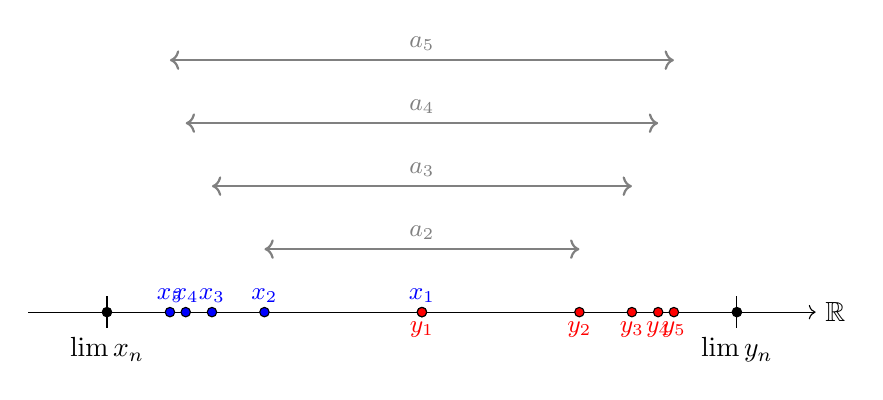
\begin{tikzpicture}[scale=2]
      % Garis bilangan
      \draw[->] (1.5,0) -- (6.5,0) node[right] {$\mathbb{R}$};
    
      % Titik batas limit
      \foreach \x/\label in {2/$\small\lim x_n$, 6/$\small\lim y_n$} {
        \draw[fill=black] (\x,0) circle (0.03);
        \draw (\x,0.1) -- (\x,-0.1);
        \node[below] at (\x,-0.1) {\label};
      }
    
      % Beberapa titik x_n dan y_n (diskalakan)
      \foreach \n in {1,...,5} {
        \pgfmathsetmacro\x{(1 + 1/\n)*2} % kalikan dengan 2
        \pgfmathsetmacro\y{(3 - 1/\n)*2}
        
        % Titik x_n
        \draw[fill=blue] (\x,0) circle (0.03);
        \node[above, blue] at (\x,0) {\small$x_{\n}$};
    
        % Titik y_n
        \draw[fill=red] (\y,-0) circle (0.03);
        \node[below, red] at (\y,-0) {\small$y_{\n}$};
    
        % Panah jarak a_n
        \ifnum\n>1
          \draw[<->, gray, thick] (\x,0.4*\n-0.4) -- (\y,0.4*\n-0.4);
          \pgfmathsetmacro\a{\y - \x}
          \node[above, gray] at ({(\x+\y)/2},0.4*\n-0.4) {\small$a_{\n}$};
        \fi
      }
    
    \end{tikzpicture}
    \caption{Ilustrasi barisan Cauchy $(x_n)$ dan $(y_n)$ di $\mathbb{R}$, serta jarak $a_n = d(x_n, y_n)$.}
    \end{figure}
\end{frame}

\end{document}